\section{Auswertung}
\label{sec:Auswertung}

\begin{figure}
  \centering
  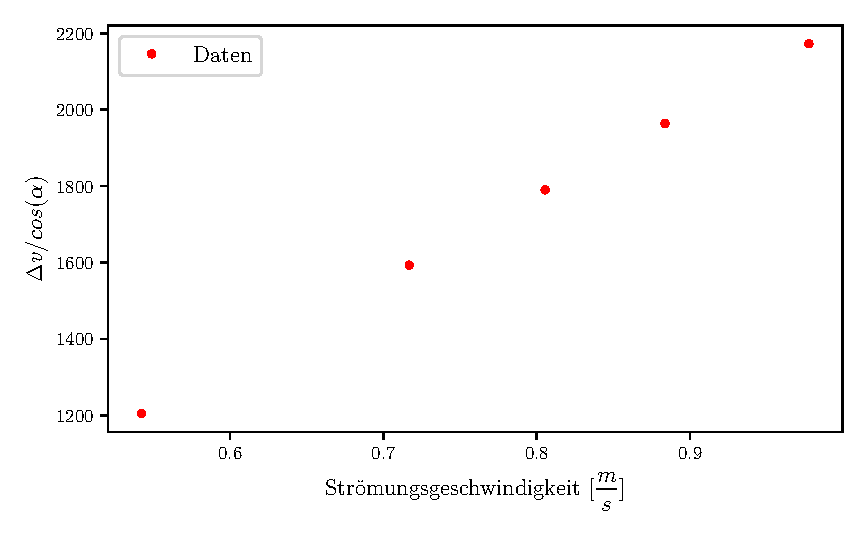
\includegraphics{plot1.pdf}
  \caption{Plot.}
  \label{fig:plot1}
\end{figure}


%T1 a,b,c =  [-5.56771465e-06  2.63829532e-02  2.93369352e+02] K/s^2, K/s , K
%errors =  [1.99814906e-07 3.84580117e-04 1.54546291e-01] 
%T2 a,b,c =  [ 4.03300677e-06 -2.08753540e-02  2.94560077e+02]
%errors =  [1.33089172e-07 2.56154288e-04 1.02937422e-01]



%dT1/dt 7 0.0230+/-0.0004
%dT2/dt 7 -0.01856+/-0.00027
%dT1/dt 14 0.0229+/-0.0004
%dT2/dt 14 -0.01862+/-0.00027
%dT1/dt 21 0.0228+/-0.0004
%dT2/dt 21 -0.01866+/-0.00027
%dT1/dt 28 0.0228+/-0.0004
%dT2/dt 28 -0.01869+/-0.00027

$cw Wasser= 4182 \si{\kilo\joule\per\kilo\gram\kelvin}$\cite[381]{PhyPrak}
%Nm= 114+/-4
%v 7 2.68+/-0.10
%vid 7 17.849999999999998
%abw 7 -85.0+/-0.6
%v 14 2.67+/-0.10
%vid 14 9.800314465408801
%abw 14 -72.7+/-1.0
%v 21 2.67+/-0.10
%vid 21 7.419392523364492
%abw 21 -64.1+/-1.3
%v 28 2.66+/-0.10
%vid 28 6.288085937500001
%abw 28 -57.7+/-1.6
%R=8.31446261815324
\begin{figure}
  \centering
  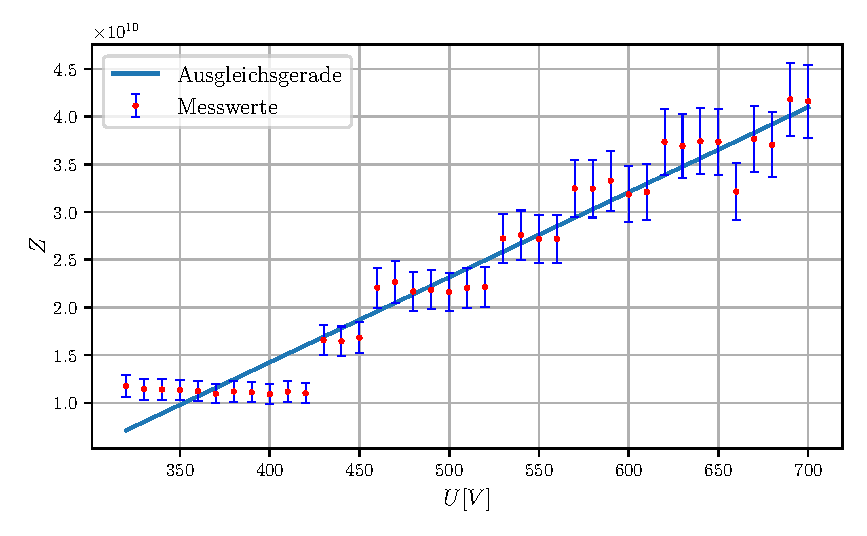
\includegraphics{plot2.pdf}
  \caption{Plot.}
  \label{fig:plot2}
\end{figure}
%a -2621.10+/-97.45
%b 10.67+/-0.31
%L 21793.07+/-810.28